\documentclass[11pt]{article}
\usepackage[margin=1in]{geometry}
\usepackage{amsmath,amssymb,amsfonts}
\usepackage{graphicx, float}
\usepackage{fancyhdr,booktabs}
\usepackage{listings}
\usepackage[normalem]{ulem}
\lstset{
    language=Python,
    basicstyle=\ttfamily\small,
    breaklines=true,
    keepspaces=true,
    showstringspaces=false
}

\renewcommand{\labelitemi}{$\bullet$}
\renewcommand{\labelitemii}{$\circ$}
\renewcommand{\labelitemiii}{$\rightarrow$}
\renewcommand{\labelitemiv}{$\cdot$}

% Header and Footer Setup
\pagestyle{fancy}
\fancyhf{}
\lhead{Ph429 NLD \& Chaos -- Fall 2026}
\rhead{Problem Set 4}
\cfoot{\thepage}

\title{\textbf{Ph429: Nonlinear Dynamics \& Chaos}\\[0.5ex]\Large Problem Set 4}
\author{Zeshui Song}
\date{Fall 2026}

\begin{document}
\maketitle

\vspace{-1em}
\subsection*{Problem 1}
In class we looked at the ``Bead on a Hoop, Submerged in Syrup'' problem. We discussed the stability of the fixed points:
\begin{align}
    x^* &= 0 && \text{top of hoop} \\
    x^* &= \pi && \text{bottom of hoop} \\
    x^* &= \pm\cos^{-1}\left(\frac{g}{r\omega^2}\right)
\end{align}
but we did not demonstrate their stability. Find their stability graphically and algebraically. Do your best.
\vspace{-1em}
\begin{center}
    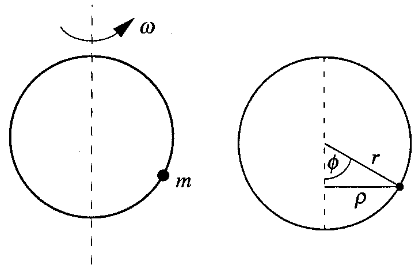
\includegraphics[width=0.45\textwidth]{bead on a hoop with GOO.png}
\end{center}

\paragraph{Solution}\mbox{}
The equation of motion for the bead on a hoop submerged in syrup is given by:
\[mr\ddot{\phi} = -b \dot{\phi} -mg\sin\phi +mr\omega^2 \sin\phi \cos\phi\]
For an overdamped system where the viscous damping dominates over inertial effects, we can neglect the inertial term (\(\ddot{\phi}\approx 0\)), leading to the first order approximation:
\[\dot{\phi} = -\frac{mg}{b}\sin\phi + \frac{mr\omega^2}{b}\sin\phi \cos\phi\]
\underline{Test for stability at fixed points:} Let $f(\phi) = \dot{\phi}$
\[f'(\phi) =\frac{df}{d\phi}= -\frac{mg}{b}\cos\phi + \frac{mr\omega^2}{b}(\cos^2\phi - \sin^2\phi)\]
\begin{itemize}
    \item \textbf{Fixed point at $\phi^* = 0$:}
    \[f'(0) = -\frac{mg}{b} + \frac{mr\omega^2}{b} = \frac{m}{b}(r\omega^2 - g)\]
    \begin{itemize}
        \item If $r\omega^2 < g$, then $f'(0) < 0$, indicating a stable fixed point.
        \item If $r\omega^2 > g$, then $f'(0) > 0$, indicating an unstable fixed point.
        \item If $r\omega^2 = g$, then $f'(0) = 0$, which is inconclusive.
    \end{itemize}
    \item \textbf{Fixed point at $\phi^* = \pi$:}
    \[f'(\pi) = \frac{mg}{b} + \frac{mr\omega^2}{b} = \frac{m}{b}(g + r\omega^2)\]
    Since $f'(\pi) > 0$, this fixed point is always unstable.
    \item \textbf{Fixed points at $\phi^* = \pm\cos^{-1}\left(\frac{g}{r\omega^2}\right)$:}\\\\
    Using the identity $\sin^2\phi = 1 - \cos^2\phi$, rewrite $f'(\phi)$ as:
    \[f'(\phi) = -\frac{mg}{b}\cos\phi + \frac{mr\omega^2}{b}(2\cos^2\phi - 1)\]
  \begin{eqnarray*}
    f'\left(\pm\cos^{-1}\left(\frac{g}{r\omega^2}\right)\right)
    &=& -\frac{mg}{b}\left(\frac{g}{r\omega^2}\right)
    + \frac{mr\omega^2}{b}\left(2\left(\frac{g}{r\omega^2}\right)^2 - 1\right)\\
    &=& \frac{m}{b}\left(-\frac{g^2}{r\omega^2} + \frac{2g^2}{r\omega^2} - r\omega^2\right)\\
    &=& \frac{m}{b}\left(\frac{g^2}{r\omega^2} - r\omega^2\right)\\
    &=& \frac{m}{br\omega^2}\left(g^2-r^2\omega^4\right)
\end{eqnarray*}
\begin{itemize}
    \item If $g^2 > r^2\omega^4$, then $\phi^*=\pm\cos^{-1}\left(\frac{g}{r\omega^2}\right)$, do not exist since $\cos^{-1}$ is only defined for values in the range $[-1, 1]$.
    \item If $g^2 < r^2\omega^4$, then $f'\left(\pm\cos^{-1}\left(\frac{g}{r\omega^2}\right)\right) < 0$, indicating stable fixed points.
    \item If $g^2 = r^2\omega^4$, then $f'\left(\pm\cos^{-1}\left(\frac{g}{r\omega^2}\right)\right) = 0$, which is inconclusive.
\end{itemize}    
\end{itemize}
\underline{Graphically testing for stability:}\\\\
Since in the stability analysis, the relationship between $r\omega^2$ and $g$ is important, I will define the parameter 
\[\lambda  = \frac{r\omega^2}{g}\] 
such that 
\[\dot{\phi} = \frac{mg}{b} \sin\phi \left(\frac{r\omega^2}{g}\cos\phi -1\right) = \frac{mg}{b} \sin\phi (\lambda\cos\phi -1)\]
Rescale time by defining $\tau = \frac{mg}{b}t$, then we have
\[\frac{d\phi}{dt} = \frac{d\phi}{d\tau} \frac{d\tau}{dt} = \frac{d\phi}{d\tau} \cdot \frac{mg}{b}\]
Using the rescaled time, we have the following first order ODE as a function of $\lambda$ and $\phi$:
\[\frac{d\phi}{d\tau} = \sin\phi (\lambda\cos\phi -1)\]
Plotting the phase portrait of $\frac{d\phi}{d\tau}$ vs $\phi$ for different values of $\lambda$ will show the stability of the fixed points.
\begin{itemize}
    \item $0<\lambda < 1$: $g > r\omega^2$
    \vspace{-1em}
    \begin{center}
        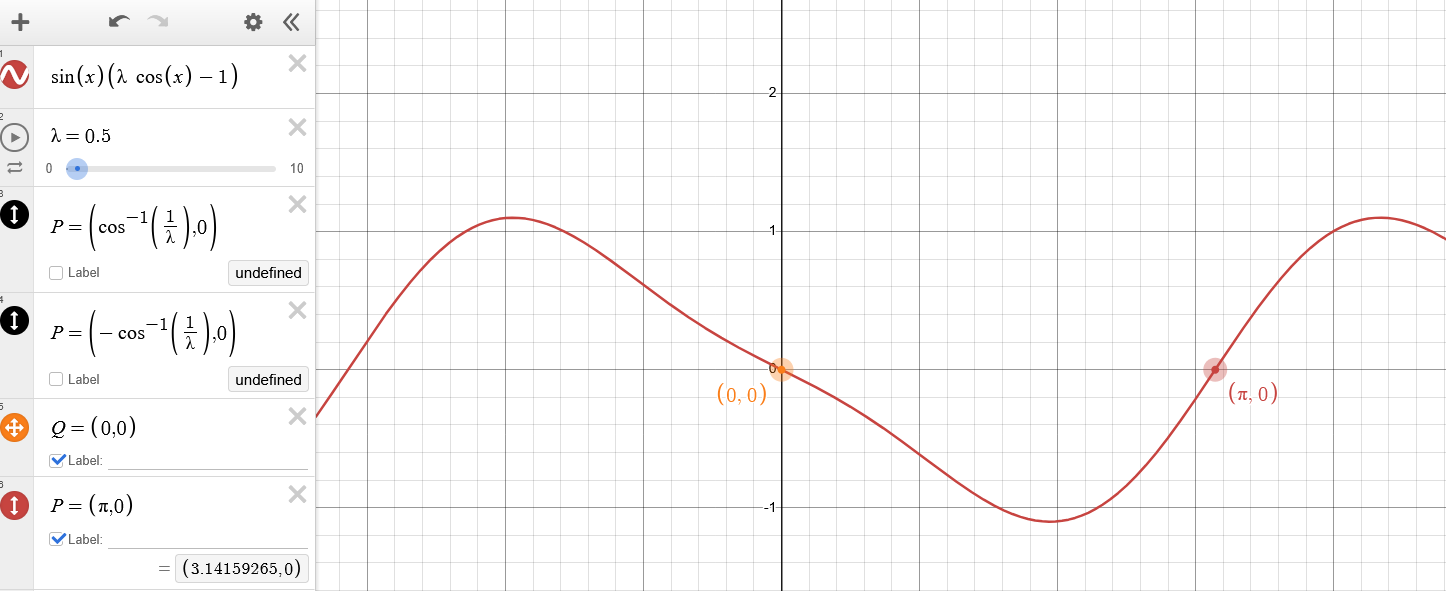
\includegraphics[width=\textwidth]{lambda l 1.png}
    \end{center}
    $\phi^* = 0$ is stable, $\phi^* = \pi$ is unstable, and $\phi^* = \pm\cos^{-1}\left(\frac{g}{r\omega^2}\right)$ do not exist.
    \item $\lambda = 1$: $g = r\omega^2$
    \vspace{-1em}
    \begin{center}
        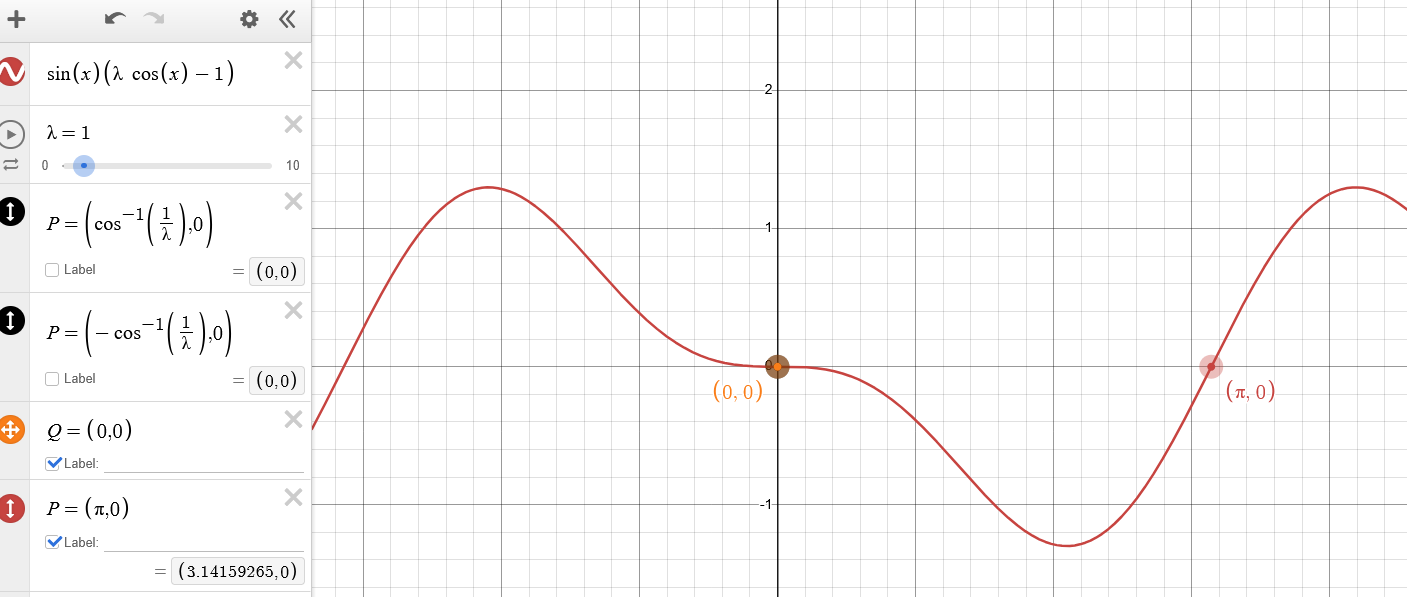
\includegraphics[width=\textwidth]{lambda e 1.png}
    \end{center}
    $\phi^* = 0$ is stable, $\phi^* = \pi$ is unstable, and $\phi^* = \pm\cos^{-1}\left(\frac{g}{r\omega^2}\right)$ coincides with $\phi^* = 0$.
    \newpage
    \item $\lambda > 1$: $g < r\omega^2$
    \vspace{-1em}
    \begin{center}
        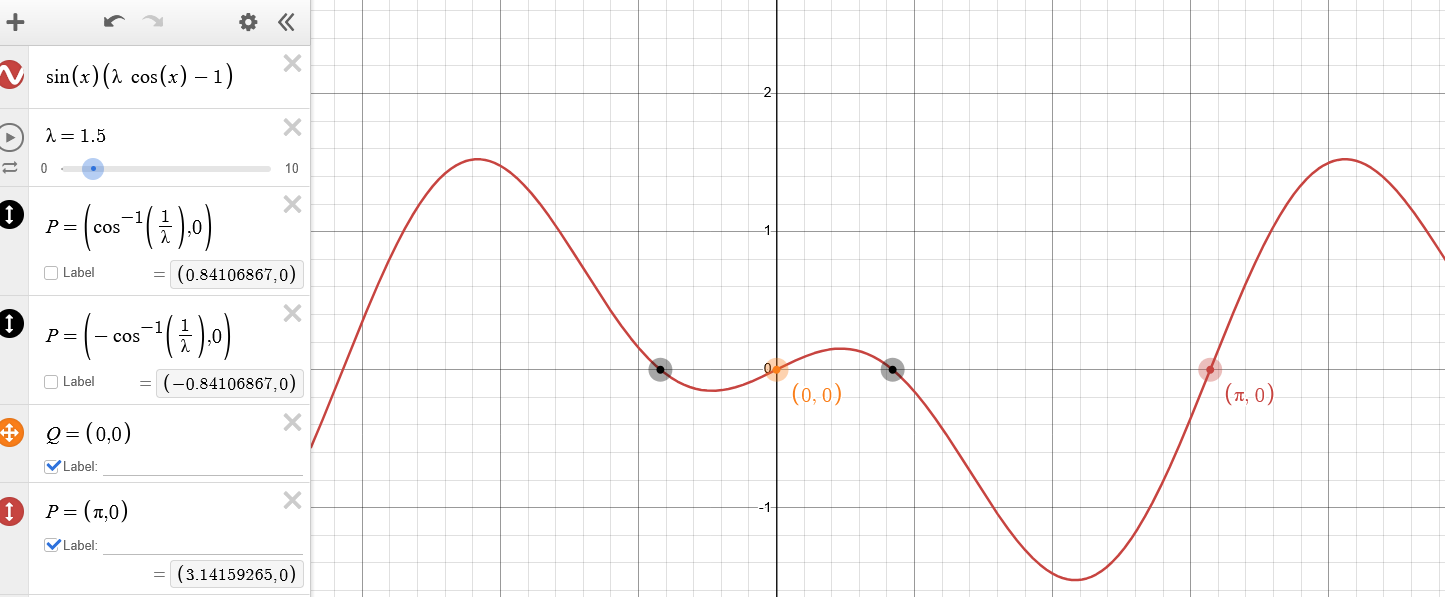
\includegraphics[width=\textwidth]{lambda g 1.png}
    \end{center}
    $\phi^* = -\cos^{-1}\left(\frac{g}{r\omega^2}\right)$ is stable, $\phi^* = 0$ is unstable, $\phi^* = \cos^{-1}\left(\frac{g}{r\omega^2}\right)$ is stable, and $\phi^* = \pi$ is unstable.
\end{itemize}
\subsection*{Problem 2}
For the following two figures, please invent a system that could produce them, giving it both in mathematical form and as a model of something (be creative, tell me a story).\\\\
\noindent\textbf{(a)}
\begin{center}
    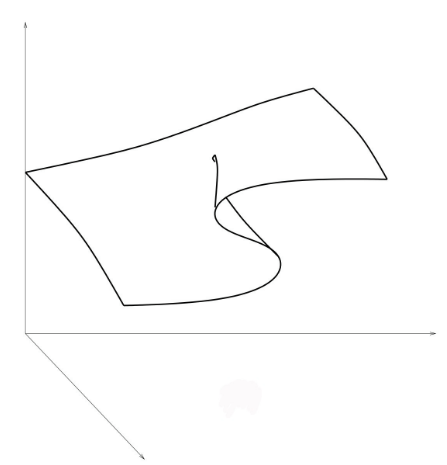
\includegraphics[width=0.38\textwidth]{p2a.png}
\end{center}
\noindent\textbf{Solution}

\vspace{2em}

\noindent\textbf{(b)}
\begin{center}
    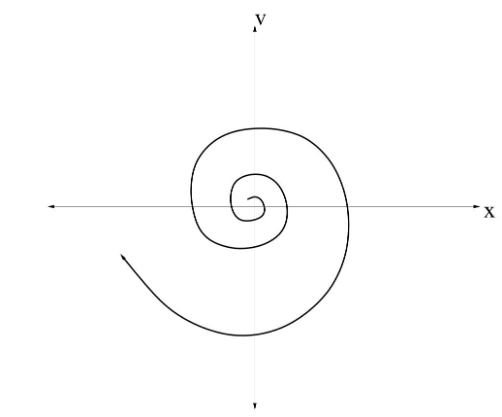
\includegraphics[width=0.38\textwidth]{p2b.png}
\end{center}
\noindent\textbf{Solution}


\end{document}